\section{Frequency Shift Keying}
\label{sec:fsk}

\subsection{Objective}

To understand the working of Frequency Shift Keying (FSK) modulation and demodulation.

\subsection{Theory}

Frequency-shift keying (FSK) is a frequency modulation scheme in which digital information is transmitted through discrete frequency changes of a carrier wave.

Logic 0 is represented by a wave at a specific frequency, and logic 1 is represented by a wave at a different frequency. The distance between logic 0 and logic 1 is known as the deviation or shift point.

\subsection{MATLAB Code}

\inputminted[fontsize=\footnotesize,autogobble]{matlab}{code/fsk.m}

\subsection{Input}


\begin{lstlisting}[language=matlab,backgroundcolor=\color{gray!10}]
>> FSK
Enter the freq of 1st sine wave carrier:
25
Enter the freq of 2nd  sine wave carrier:
50
Enter the freq of periodic Binary Pulse (Message):
25
Enter the amplitude (both carrier and binary pulse message):
5
\end{lstlisting}

\subsection{Output}

\begin{figure}[ht]
    \centering
    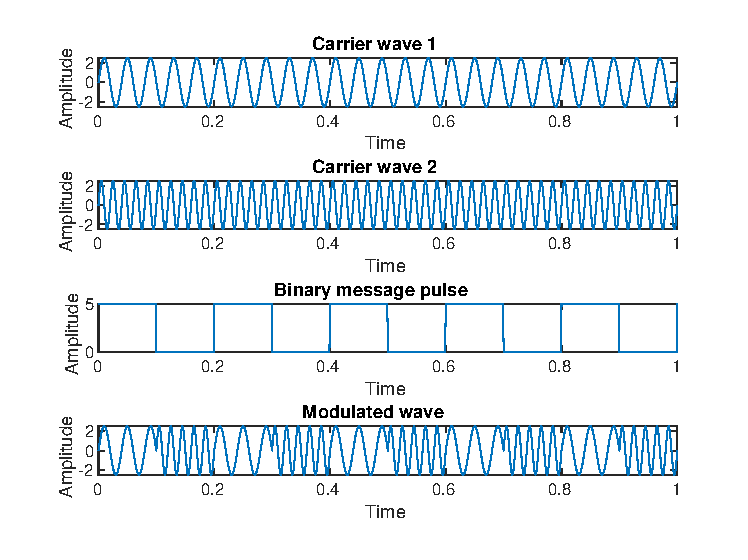
\includegraphics[width=0.8\textwidth]{res/figures/FSK.pdf}
    \caption{FSK Modulation}
    \label{fig:fsk}
\end{figure}